% options:
% thesis=B bachelor's thesis
% thesis=M master's thesis
% czech thesis in Czech language
% slovak thesis in Slovak language
% english thesis in English language
% hidelinks remove colour boxes around hyperlinks

\documentclass[thesis=M,english]{FITthesis}[2012/06/26]

\usepackage[utf8]{inputenc} % LaTeX source encoded as UTF-8

\usepackage{graphicx} %graphics files inclusion
% \usepackage{amsmath} %advanced maths
% \usepackage{amssymb} %additional math symbols

\usepackage{dirtree} %directory tree visualisation

% % list of acronyms


\usepackage[acronym,nonumberlist,toc,numberedsection=autolabel]{glossaries}
\iflanguage{english}{\renewcommand*{\acronymname}{List of abbreviations used}}{}
\makeglossaries

\usepackage{todonotes}
\usepackage{enumitem}
\usepackage{hyperref}
\usepackage{tabularx}
\usepackage{spverbatim}
\usepackage{listings}
\usepackage{caption}
\usepackage{adjustbox}

\DeclareCaptionFont{white}{\color{white}}
\DeclareCaptionFormat{listing}{\colorbox{gray}{\parbox{\textwidth}{#1#2#3}}}
\captionsetup[lstlisting]{format=listing,labelfont=white,textfont=white}

\newcommand{\tg}{\mathop{\mathrm{tg}}} %cesky tangens
\newcommand{\cotg}{\mathop{\mathrm{cotg}}} %cesky cotangens

\department{Katedra \ldots softwarového inženýrství}
\title{A Case Study and Proof of Concept of the Application of Machine Learning to Polarion's ALM Software}
\authorGN{Michal} %(křestní) jméno (jména) autora
\authorFN{Sláma} %příjmení autora
\authorWithDegrees{Bc. Michal Sláma} %jméno autora včetně současných akademických titulů
\author{Michal Sláma} %jméno autora bez akademických titulů
\supervisor{Ing. Jurij Černikov}
\acknowledgements{I would like to thank to my supervisour for his extraordinary leading and valuable advices during the whole process of writing this thesis.}
\abstractCS{Diplomová práce obsahuje přehled možný požití stojového užení v aplikace Polarion ALM. Práce začíná analýzou funkcí Polarionu následovanou recenzí nejběžnějších \acrshort{ml} frameworků a algoritmů vhodných pro použití v prostředí Polarionu. Následuje popis důležitých případů použití s cílem najít nejvhodnějšího kandidáta pro aplikaci \acrshort{ml}. Pro dva vybrané případy použití je vytvočen prototyp s využitím produkčních dat a následně je důskutována náročnost budoucího nasazení do produkce spolu s komplikací ve formě nové \acrshort{gdpr} směrnice.}
\abstractEN{Master thesis contains an overview of possible ways how to use Machine learning (ML) in Polarion ALM software. Thesis begins with analysis of Polarion functionality is followed by review of \acrshort{ml} frameworks and algorithms suitable for using in Polarion environment. Followed by description of important user cases with business value and appropriate for \acrshort{ml} implementation. By combining the previous one two user cases are selected to create a prototype based on production data. Finally we are discussing deployment to production and its problems including new \acrshort{gdpr} regulation.}
\placeForDeclarationOfAuthenticity{V~Praze}
\declarationOfAuthenticityOption{4} %volba Prohlášení (číslo 1-6)
\keywordsCS{Strojové učení, životní cyklus softwarových aplikací, ALM, GDPR, AWS, Amazon web services, LDA, Latent Dirichlet allocation}
\keywordsEN{Machine learning, application lifecycle management, ALM, GDPR, AWS, Amazon web services, LDA, Latent Dirichlet allocation}

\begin{document}

\newacronym{alm}{ALM}{Application lifecycle management}
\newacronym{plm}{PLM}{Product lifecycle management}
\newacronym{ml}{ML}{Machine learning}
\newacronym{polarion}{Polarion}{Polarion ALM} 
\newacronym{pof}{PoF}{Proof of Concept} 
\newacronym{rnn}{RNN}{Recurrent neural network}
\newacronym{aws}{AWS}{Amazon web services}
\newacronym{gui}{GUI}{Graphic user interface}
\newacronym{cntk}{CNTK}{Microsoft Cognitive Toolkit}
\newacronym{lda}{LDA}{Latent Dirichlet allocation}
\newacronym{gdpr}{GDPR}{General Data Protection Regulation}
\newacronym{ocr}{OCR}{Optical character recognitionn}
\newacronym{d3}{D3}{Data-driven documents}
\newacronym{saas}{SaaS}{Software as a service}


\todototoc
\listoftodos

\begin{introduction}
\begin{center}
	\textit{“The revolution is just beginning, but it’s real – and the time to act is now. In fact, it is yours for the taking to harness a broad platform, services and ecosystem to transform your business. A unified approach to application lifecycle management is not a futuristic technology trend. It’s here today,and the good news is that you don’t have to completely stop and reset, but can smoothly transition from squeezing the most out of your existing business processes to making your organization thrive.“}\\
Kurt Bittner\\
Analyst\\
Forrester Research\\
\end{center}
\end{introduction}

Author of this thesis has been working in software development for more than 10 years. Based on this experiences he got to a question how to manage and keep up to date info for large project where more than dozens people are involved. This is also why he chooses to work as a developer of \acrshort{polarion}.


We live in the world that is changing rapidly. No part of life of free to this changes and the software development needs more then others to adapt every day to new requirements and technologies. This demand leads to a new level of management for software development where tools, process, implementation, testing and reporting are organized on one place with goal to keep and improve traceability and productivity as high as possible. This comes hand by hand with automation in the form of \acrshort{ml} that moves user experience and reporting to the next level. One of such product is \acrshort{polarion}\cite{polarion_alm} and this work will analyze it's user cases and find out what places are good candidates for using \acrshort{ml} techniques to improve business value of the product. 

\chapter{The aim of the thesis}

The aim of this thesis is to analyze and identify machine learning (\acrshort{ml}) use cases that would prove valuable for \acrshort{polarion}’s application lifecycle management (\acrshort{alm}) software. A proof of concept prototype will be supplied for the selected use case.

\begin{enumerate}[nosep]
	\item Analyze and describe \acrshort{polarion} in order to identify suitable use cases to apply ML to. 
	\item Provide a review of ML frameworks and algorithms that are relevant for such an application.
	\item Describe several use cases for ML and define their benefit to both \acrshort{alm} as a business and the users that deploy it.
	\item Choose a scenario from the previous investigation and implement a proof of concept prototype.
	\item Discuss the possibility of the full implementation and deployment of the previous prototype into the production environment.
\end{enumerate}

\chapter{Polarion}

Organizations are often struggling with the old processes of doing things. They focus on isolated process optimization instead of driving
business value through comprehensive synchronization. With \acrshort{polarion}, customers have been able to get their teams out of their silos and orchestrate development efforts across the entire application lifecycle. This approach has empowered stakeholders to better perform tasks in context and quickly make sound decisions based on real-time access to information.\\

You can try \acrshort{polarion} on \url{https://polarion.plm.automation.siemens.com/}.\\

Now let's take a look what \acrshort{polarion} comes with and how improves old fashion processes.


\section{ALM}

\begin{center}
	\textit{“ALM is a paradox in the software engineering
		world, where engineers recognize
		the need for requirements management,
		change and configuration management, QA
		and test management, and so on, but are
		not familiar with the term ALM. This is a
		serious problem because ALM is necessary
		to manage software complexity, and the rise
		of embedded software in engineered products
		needs mature management processes
		and tools.”}\\
	Michael Azoff\\
	Principal Analyst\\
\end{center}

\acrshort{polarion} is a \acrshort{alm} enterprise solution to deal with modern-day challenges. It has emerged with the intent to fasttrack
innovation, while safeguarding quality, functional safety and compliance to satisfy that speed in developing and delivering innovative applications is becoming essential to the success of businesses in any industry.\\

\pagebreak
\acrshort{alm} points to these three aspects:
\begin{enumerate}[nosep]
	\item application has to be delivered as fast as possible and the time is a new strategy weapon 
	\item information technologies are fuel accelerating business success
	\item errors are not forgiven and can go viral in instant. QA rules must be set and obeyed.
\end{enumerate}

\section{A unified solution}

\acrshort{polarion} is a single solution providing a solution to build whole application from the ground. At the same time it is ensured that data and logic is in persistent state during entire process.\\ 

This helps with regulations. This basic word means a lot in the world of software development where processes are regulated by intern or external subject and have essential impact on the cost of product not only during development but after it's release.\\

What \acrshort{alm} comes with?\\

The main advantages attributed to ALM process (graphically shown in the picture \ref{fig:alm_unified_solutionc}):
\begin{itemize}[nosep]
\item Agility through improved collaboration.
\item Productivity through process integration.
\item Auditability through traceability and accountability.
\item Quality through transparency and automation.
\item Innovation through unlocked team synergy.
\item Predictability through better estimation and reporting.\\
\end{itemize}

\begin{figure}[h!]\centering
	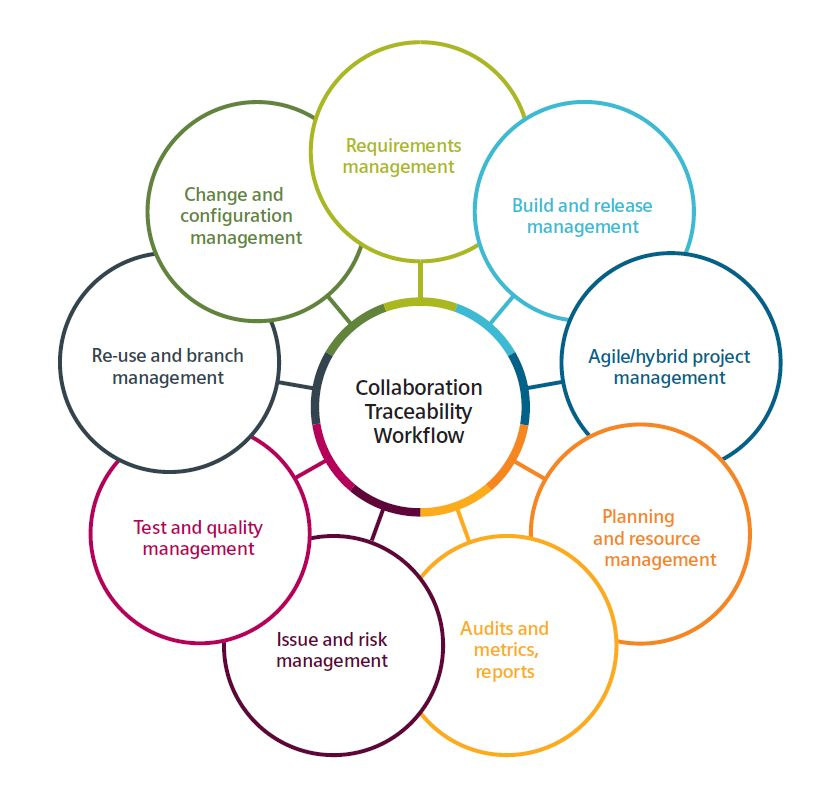
\includegraphics[width=1\textwidth]{pictures/alm_unified_processes}
	\caption{A unified solution for ALM \cite{polarion_alm}}\label{fig:alm_unified_solutionc}
\end{figure}

Let's a look more close to some of these advantage.

\subsection{Agility through improved collaboration}

If faster time-to-market is a key success factor in today’s competitive environment, real-time collaboration and contextual performance 
of tasks are the means to stay ahead. In many cases, lightweight Agile software development methods have replaced or augmented incremental waterfall methods to release products more frequently.\\

\acrshort{polarion} provides flexible support for Agile or Lean, as well as traditional and hybrid environments, including any customized Scrum, feature-driven development, Kanban, extreme programming, or rational unified process methodologies.\\

The \acrshort{polarion} 100 percent browser-based architecture makes information universally accessible from anywhere for any collaborator. Collaboration is so easy and teams divided around the world can communicate to each other and solve tasks together.\\

\subsection{Productivity through process integration}

Major part of \acrshort{polarion} customers apply a combination of Agile and DevOps methodologies The \acrshort{polarion} solution is the perfect conduit to DevOps, allowing easy synchronization of development and delivery processes spanning requirements definition, feature development, quality testing, and maintenance. Any problem can be easily tracked back to the source and time of maintenance is so rapidly reduced even to real time fixes.

\acrshort{polarion} supports integration with other tools. This is done by extension or native integration. Thanks this customers can still use their own tools and data repositories and just integrate them with \acrshort{polarion}. \acrshort{polarion} has it's place on market for many years and during this time many extensions were created by customers or professional services and placed to official \acrshort{polarion}'s marketplace from which can be freely downloaded. Common customer will find there with high probability a solution for his needs.  

\subsection{Auditability through traceability and accountability}

\begin{center}
	\textit{“We chose Polarion ALM at Phoenix Contact
		in the Business Unit Automation to consolidate
		our very heterogeneous tool
		landscape – PVCS, Bugzilla, OneTree. With
		Polarion ALM we achieved transparency on
		all levels of development and we got fast
		acceptance in the teams. We now see exactly
		and in detail the status and the progress in
		our projects in the different project phases.”}\\
	Andreas Deuter\\
	Phoenix Contact Electronics\\
\end{center}

Every change is stored. \acrshort{polarion} stores all you need to track down what, how and by whom happened. In enterprise environment where is working hundreds and hundreds people it's hard to keep in touch who does what. A place where you see it all is priceless and helps to minimize risks of black holes when tasks is left or forgotten without any notice. Such a missing task can have very serious impact on cost or even release date itself.  

\subsection{Quality through transparency and automation}

A big problem with this approach is that team members usually get the information about what they need to accomplish from static documents that tend to go out-of-date as quickly as they were created. But perhaps worst of all, changes and ad hoc decisions often fail to take into account the downstream impact.\\

Processes of \acrshort{polarion} provide way to track all requirement changes and so help to keep in touch with actual state of what needs to be done. For instance if product owner change a task developer is informed and can react by accepting this task or request more information about this change. In both cases every side knows what happened and what comes next.\\

Time when all operations were done only by people is over and automation plays important role in IT management. \acrshort{polarion} provides environment to run automatic jobs to build, test, check, ... or whatever customer may need. Customers are free to implements their own job and run them in the same way as native ones.

\subsection{Automating proof of compliance}

On the most important aspect is document workflow and will need this further in thesis.\\ 

You can understand to document as a normal word document but each task (in \acrshort{polarion} called work item) is external object. That means document is composed from its own text (headings, descriptions...) and work items that also have its description which is shown in the document. All theses together makes customer feel that is working with one unit. If customer wants to edit work item this can be done on document or via work item view easily accessible from document or another part of \acrshort{polarion} as working with work items is the main activity and processes are built on them. Let's look at the workflow shown in \ref{fig:document_workflow}.

\begin{figure}[h!]\centering
	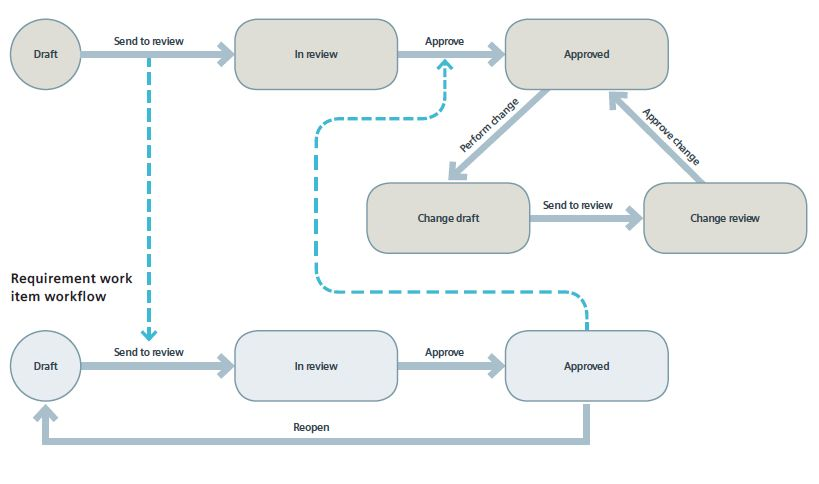
\includegraphics[width=1\textwidth]{pictures/document_workflow}
	\caption{Document workflow \cite{polarion_alm}}\label{fig:document_workflow}
\end{figure}

Picture \ref{document_workflow} shows two separated workflows. One for document and one for work items. Workflows itself does not need explanation but the important part is the relation between them. Document can not move to a next state unless all it's work items are also moved to a desired state. This keep traceability and collaboration consistence by pushing team to accept it's work and remove not desired drafts, fakes and other stuff that is not related to real work. 

\subsection{Innovation through unlocked team synergy}

We live in information age. Information are all around us and the hardest part is to find what is important for us or company and what can be forgotten. Team is a great way how to share this information but what if team has many people? \acrshort{polarion} contains way how to cooperate and improve your know how as fast possible and share it with other co-workers. Time to solve already solved issued is rapidly reduced and new task can be done based on results of previous work that leads to more accurate estimations and risk assessment.

\section{Development process in complex or regulated environments}

Most collaborators don’t have the unified tools environment necessary to get them on the same page at the same time, however, and resulting disconnects have increasingly negative impact, disrupting industries with new records of regulatory warning letters, product failures, recalls, legal sanctions, loss in market position and associated cost explosions.\\

Topping the list of challenges in the new world of software driven innovation are the need for tight orchestration across disparate teams, growing regulatory demands and the increasing role of suppliers as innovation partners. Companies that are able to shift gears to meet the growing complexity will be well positioned to secure new market opportunities.

Common first step is to welcome agile approach. Companies have different expectations about it's benefits shows in the picture below \ref{fig:agile_benefits}.

\begin{figure}[h!]\centering
	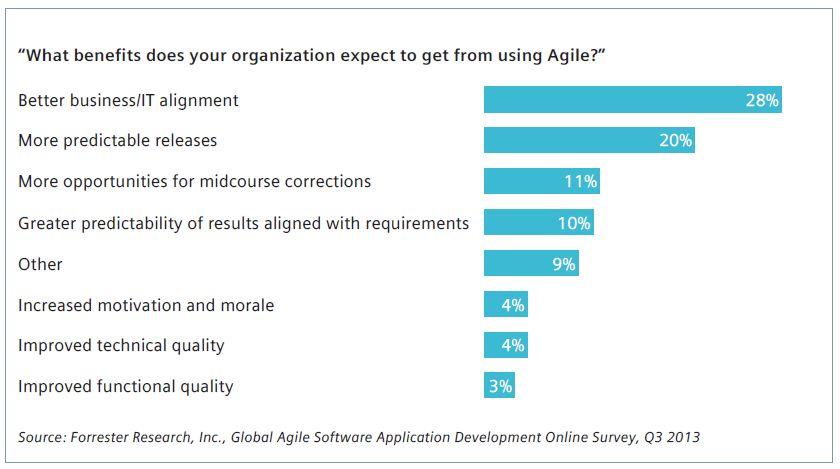
\includegraphics[width=1\textwidth]{pictures/agile_benefits}
	\caption{Companies expectation from using Agile\cite{polarion_alm}}\label{fig:agile_benefits}
\end{figure}

Result is clear. Companies feel that IT is starting to be more and more complex and demands from business is harder to satisfy. \acrshort{polarion} support all agile methods and is ready to help company improves its environment. More importantly this agile templates (how are called) can be modified based on customers demands to fit their needs and specify requirements.

\begin{center}
	\textit{“Siemens PLM Software’s Polarion
		products presents the opportunity to
		allocate our complex and formal
		development rules via one state-of-theart
		tool. The modularity and flexibility
		make the adjustment to our needs simple
		and effective. The traceability and
		workflow features are convincing and
		really assist the everyday activities.”}\\
Christian Kettl\\
MTU Aero Engines\\
\end{center}

\subsection{Integration of ALM and PLM}

All the time we are talking about \acrshort{alm} but the main goal is to provide entire solution for product application lifecycle \acrshort{plm} where \acrshort{alm} is just a part of it. Where \acrshort{alm} is concentrated around application there \acrshort{plm} is the process of managing the lifecycle of a product itself from inception to final real item. \acrshort{polarion} is able to provide this functionality by integration with external tool that can use \acrshort{polarion} as the source of \acrshort{alm} work flow.\\

ALM-PLM integration benefits include:

\begin{itemize}[nosep]
	\item Integrated processes make cross-discipline synchronization
	very easy.
	\item Access to product and software requirements supports
	comprehensive understanding of the product definition.
	\item Bi-directional linking enables cross-discipline lifecycle
	management and audit readiness.
	\item Change propagation and automatic notification enable
	comprehensive change impact analysis.
	\item Synchronized testing and reporting support cross-functional
	defect management.
	\item Linked, versioned data architecture without data duplication
	delivers closed-loop decision making.
	\item Integration makes holistic compliance reporting for every
	aspect of the manufacturing process a reality.
\end{itemize}

\section{Accelerate collaboration}

Development environments to synchronize team efforts have proliferated. But most of them are cobbled together, posing a wide range of disadvantages. Leveraging \acrshort{polarion} flexibility, customers can choose from different configurations to provide all collaborators with the level of information and functionality they need, while keeping the total cost of ownership the lowest in the industry.

These are the most common:
\begin{itemize}[nosep]
	\item Difficulty linking and tracing artifacts across differently
	structured repositories.
	\item Problems of low visibility into project status, impact of
	changes and release predictability.
	\item Lack of a cohesive feedback loop that brings important
	context to every stakeholder.
\end{itemize}

\begin{figure}[h!]\centering
	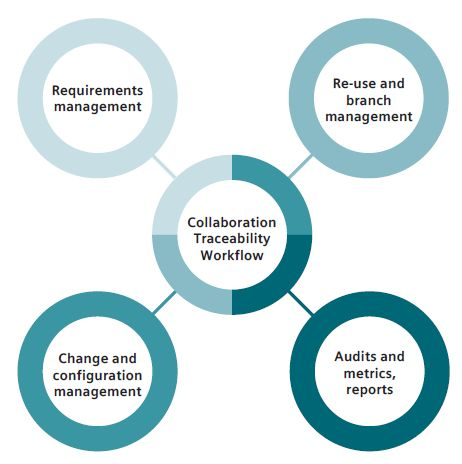
\includegraphics[width=1\textwidth]{pictures/collaboration_workflow}
	\caption{Collaboration traceability workflow \cite{polarion_alm}}\label{fig:collaboration_workflow}
\end{figure}

\subsection{The dilemma of requirements documentation}

We need to be sure that all side speaks with dialect that respect specify domain. This requirement typically encompass varying pieces of content, including:
\begin{itemize}[nosep]
	\item Paragraphs to provide overviews and explain details.
	\item Lists and tables to detail structured data and rules.
	\item Images and models to illustrate requirements.
	\item Flow charts to describe a series of events.
\end{itemize}

\subsection{"easy-as-Word functionality"}

If we spoke that the base object in \acrshort{polarion} is Document we shall expect that customers will use document in the same way as if they were using in the Microsoft Word. Fortunately behaviour of document in \acrshort{polarion} is very similar in both using and how looks like.\\

Customers can use known buttons and tools from Microsoft Word to edit and interact with document and this speed up learning curve a lot. 

\subsection{Real-time access to content}

Instead of Microsoft word document is \acrshort{polarion} document fully online and each change is immediately visible to everyone. Many users can simultaneously edit one item and \acrshort{polarion} then handle merging of changes. Of course that this can lead to conflict and in this case user have to handle his changes by own.\\ 

Consequently, companies that use Polarion Requirements are no longer forced to rely on meetings, sending emails, or circulating formal documents to make decisions, even with their partners and other external collaborators.

\subsection{Tie in domain experts with their tools}

As was said previously \acrshort{polarion} is expandable. Extensions can change or improve some existing functions or add completely new, transfer data from or to \acrshort{polarion} or connect it to external tools providing new functionality.\\

To complete the picture, connectors for popular third-party tools such as HP® Quality Center® and Atlassian® Jira® are available, and so is an open and fully documented Java API. As a result, a strong community of more than 100,000 members has formed and created extensions, integrations and customizations.

\subsection{Deliver release predictability}

Because every artifact change in the Polarion product is tracked and reported using the underlying configuration management system, customers automatically gain a complete audit trail of who did what, when and why, making it impossible to change anything without leaving a trace.\\

“Visual Diff” functionality is available to easily detect the changes between different states, and customers report that teams that take advantage of change management and impact analysis are much more successful.

\subsection{Reduce time-to-marker}

All previous parts have one main purpose to deliver product in the shortest time but ensure its quality and traceability.\\
 

\section{Medical domain}

One the strongest part of \acrshort{polarion} is in ability to satisfy regulation demands from various types of institutions that making development more complex then before. \\

Lets talk about medical domain.\\

Medical device product development work is a highly integrated and regulated process. Two key standards incorporated into medical device risk management are International Organization for Standardization (ISO) 14971:2009, which specifies the process for a manufacturer to identify the hazards associated with medical devices; and ISO Technical Information Report (TIR) 24971:2013, which provides guidance in addressing specific areas of ISO 14971 when implementing risk management. Europe has added to the mix with EN ISO 14971:2012, which is different in several important aspects, and is required if a company is selling medical devices into Europe. You can see this process in Medical risk management workflow picture \ref{fig:medical_standard}.\\

It was just a example how problematic and regulated this domain is.\\

\begin{figure}[h!]\centering
	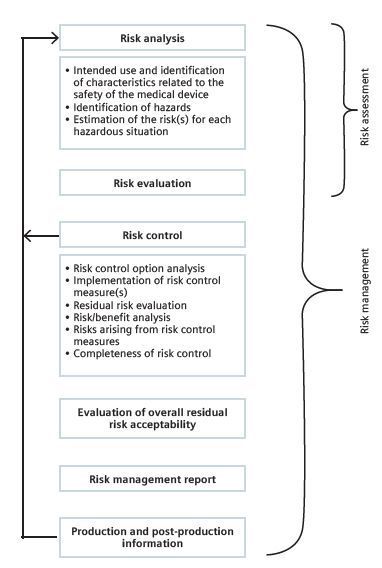
\includegraphics[width=1\textwidth]{pictures/medical_standard}
	\caption{Medical risk management workflow \cite{polarion_alm}}\label{fig:medical_standard}
\end{figure}

To describe how exactly is \acrshort{polarion} used in medical domain s beyond the scope of this thesis. But one point are data. Data are in medical domain valuable asset whose using is restricted by law and violation has serious financial and social impart. If we want to use this data we have to be use that all rules are obeyed and data are safe before abuse or stolen.

\chapter{Machine learning}

It's over 50 years since the first mention of \acrshort{ml} by Arthur Lee Samuel in his study \textit{Some Studies in Machine Learning Using the Game of Checkers}\cite{ml_first_occurence}. At that time it was just an idea IT was not ready to support it. But now we are fully in information age. Machines are able to calculate incredible fast and we are able to store all data what we need. From this \acrshort{ml} has risen and companies from every corner domains have realised that \acrshort{ml} can improve their product significantly or even create entirely new ones.\\

The path from just a theory to practical usage was long and hard \cite{ml_history}.\\

\begin{itemize}[nosep]
	\item 1979 — Students at Stanford University invent the “Stanford Cart” which can navigate obstacles in a room on its own.\\
	- If you at it from today the achievement is a bit funny but on the other hand it is almost 40 years old.
	\item 1997 — IBM Deep Blue Beats Kasparov\\
	- You sure remember this event. It was also  moment when author of this thesis heard about \acrshort{ml} for the first time along side with public. Machines stopped to be perceived just like calculators and got a status of thinking think.
	\item 2016 — Beating Humans in Go\\
	 - Google's AlphaGo was able to beat professional human player using a combination of machine learning and tree search techniques. What will be next? 
\end{itemize}

\pagebreak
During MLP 2018 \cite{mlp2018_microsoft} was presented a heartbreaking user case for face recognition. Try to imagine nature disaster leading to thousands and thousands refugees. Families are divided and with all that chaos around it is impossible to find each other. Depression is rising and may lead to panic or violence on himself or someone else. \acrshort{ml} comes with simple idea. Just take a picture of yourself and it will find your relatives. How? \acrshort{ml} has learnt on data from other families and find out what common family characters are and how can be used. Based on this \acrshort{ml} is able to say with high probability if someone is related to someone. \\

What makes this examples so special? This user case uses \acrshort{ml} in a new way but algorithms and frameworks were already here. Data was provided, model was created and it works. Sounds pretty easy and of course reality was a bit complicated but leave us a message where the current state of \acrshort{ml}. Companies can use existing implementations without deep knowledge of complicated algorithms and may straightly start with their own problems, business case and see results in a short time.\\

It was said that with using of existing solutions \acrshort{pof} should not take more than 2 months according to learning task and processed data.

Learning can be done in different ways: 
\begin{itemize}[nosep]
\item Supervised learning: relies on data where the data are annotated and algorithm comes through them and tries to find similarities. For example, we want to distinguish between pictures of cats and dogs. Algorithm will go through on lots of annotated pictures and classify them. After it algorithm will be able correctly annotated new pictures but the main disadvantage is need of a large amount of preprocessed data. 
\item Semi-supervised learning: algorithm does not have any annotations. Again a large amount of data are provided to algorithm and with some characteristics what we want to find. In our case of cats and dogs we want to separate pictures into two groups. During this separation algorithm will learn rules how cats and dogs look like. Compared to the previous one we are good with raw data and no preprocessing is needed.
\item Reinforcement learning: Chess play is good example of this learning when want to win. Algorithm gets set of plays with moves and results and it learns on this trying to find best moves leading to victory. In case of games this approach has a great advantage that algorithm can play with himself and play many games in a short time that is for people question of minutes or hours.
\end{itemize}


For the first Let's see what \acrshort{ml} frameworks or libraries are available.

\section{TensorFlow}

TensorFlow\cite{ml_tensorflow} is an open source software library with strong support for machine learning and deep learning and the flexible numerical computation core is used across many other scientific domains. Developed by Google for its internal usage but fast became one the most used \acrshort{ml} framework. The reason for this is the ease with which developers can build and deploy applications.

Main focused is on deep learning and has more tools to support reinforcement learning and other algorithms. Deep learning concept is shown in the figure \ref{fig:ml_tensorflow_dl}.

\begin{figure}[h!]\centering
	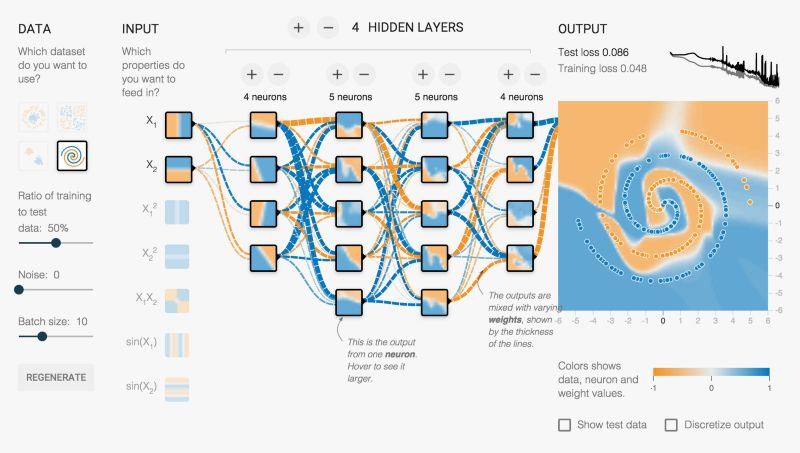
\includegraphics[width=1\textwidth]{pictures/ml_tensorflow_dl}
	\caption{Deep learning concept of Tensorflow \cite{ml_tensorflow_dl}}\label{fig:ml_tensorflow_dl}
\end{figure}

Tensorflow has much better performance and customizability, but the learning curve is much steeper as you are not just plugging in data and labels into a constructor, but are actually creating the layers which will make up your model. For its using you need solid understanding of machine learning and mathematical concepts especially linear algebra and calculus.
\pagebreak

\section{PyTorch}

A Python version of Torch, known as Pytorch, was open-sourced by Facebook in January 2017. It is based on dynamic computation graphs. This has a lot of useful benefits for certain types of \acrshort{rnn}, situations where you need to generate weights and things where the very structure of the network changes.\\

PyTorch\cite{ml_pytorch} also has a really nice interface and has the support of Facebook. And contains lots of modular pieces that are easy to combine. The downsides are that it’s a relatively newer framework, so there’s not many integrations with it, not much community and not many papers implemented in it. And note that dynamic computational graphs will make many things rather inefficient because lacking static optimizations.

\section{Keras}

Keras was created by Francois Chollet, a software engineer at Google and is a deep-learning library that sits atop TensorFlow and Theano, providing an intuitive AP that is inspired by Torch and its development is fast growing.\\

On the other hand as Keras\cite{ml_keras} is good in rapid prototyping it lack in flexibility.

\section{Caffe2}

Caffe2\cite{ml_caffe2} with C++ engine is a successor to the original Caffe and is the second deep-learning framework to be backed by Facebook after Torch/PyTorch. The main difference is that Caffe2 is more scalable and light-weight but rather limited in flexibility. Good for smartphone inference.

\section{Amazon web services}

\acrshort{aws} provides a low-cost, scalable and highly reliable infrastructure platform in the cloud. This has been adopted by thousands of businesses globally. Australia, the US, Japan, Europe, Singapore and Brazil are among the data center locations. The locations are widespread to make sure the system is robust and secured against the impact of outages or other such problems.\\

Advantages\cite{ml_aws_advantages} 
\begin{itemize}[nosep]
	\item Security.\\
-\acrshort{aws} conducts regular audits to ensure its infrastructural security. It has implemented best practices in security and also provides documentation on how to deploy the security features. It ensures the availability, integrity and confidentiality of your data and provides ‘end to end’ privacy and ‘end to end’ security.
	\item Cost-Effectiveness\\
-You consume only as much storage or computing power as required. No upfront investment or minimum expenditure is required. Generally, it is not easy to predict the requirements for the resources. So, you might allocate fewer resources than required and impact customer satisfaction or you might allocate excessive resources and not be able to maximize return on investment (ROI).
	\item Flexibility and Openness\\
- You can use the programming languages, architectures, operating systems and databases you are familiar with. In this manner, there won’t be any need for your IT personnel to pick up new skills and the overall time to market and productivity will improve. 
	\item Elasticity and Agility\\
- allows you experiment and innovate quickly through its huge global cloud infrastructure. You can quickly scale up or scale down on the basis of demand. You can also use new applications, rather than wait for months for hardware.\\
\end{itemize}

Common company solves a problems those can be group by\cite{ml_aws_benefits}
\begin{itemize}[nosep]
\item Overspending on hardware and storage capacity. 
\item Business leaders want IT to help preserve cash. 
\item A non-standardized IT environment and platform is expensive from a  security, support and training perspective.\\
\end{itemize}

All these problems are solved by \acrshort{aws}.\\

\acrshort{aws} provides wide range of services shown in the picture below \ref{fig:ml_aws_sagemaker_stack}.

\begin{figure}[h!]\centering
	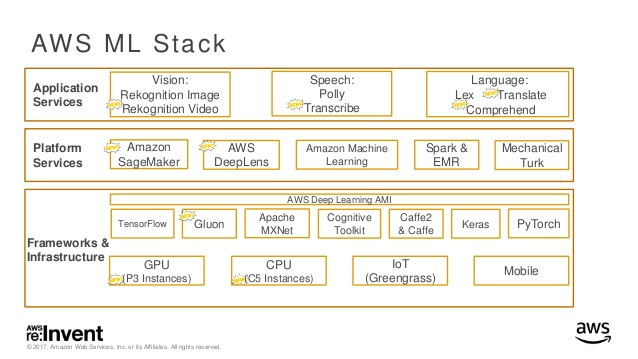
\includegraphics[width=1\textwidth]{pictures/ml_aws_sagemaker_stack}
	\caption{AWS ML stack \cite{ml_aws}}\label{fig:ml_aws_sagemaker_stack}
\end{figure}

\subsection{Frameworks and infrastructure}

At the low end computation customers can choose from the most used frameworks:
\begin{itemize}[nosep]
	\item Mxnet 
	\item TensorFlow 
	\item Caffe2
	\item Keras
	\item CNTK
	\item PyTorch
	\item Gluon
\end{itemize}

Using is then just about calling united interface without dependence with framework was chosen. It bring great for testing different approaches in a short time.

\subsection{Application services}

It is SaaS layer with applications ready for use. Customers do not need to implement their own solutions to test their data in common cases and can start to use it immediately.


\subsection{Platform services}

On this level resides what we can expect except one and this is Amazon SageMaker.

Amazon realized that developers need a fast way how to build, train and deploy machine learning models with as litter effort as possible. And for this purpose SageMaker was created.

Let's look closer on Amazaon SageMaker.

\subsection{SageMaker} 

Amazon SageMaker is a fully-managed platform that enables developers and data scientists to quickly and easily build, train, and deploy machine learning models at any scale with easy to use \acrshort{gui}.\\

\begin{figure}[h!]\centering
	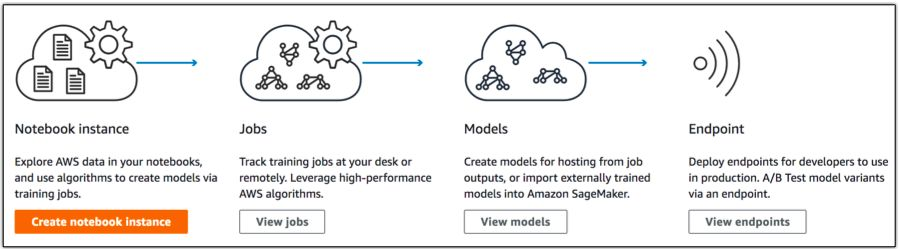
\includegraphics[width=1\textwidth]{pictures/ml_aws_sagemaker_buildprocess}
	\caption{Amazaon machine learning stack \cite{ml_aws}}\label{fig:ml_aws_sagemaker_buildprocess}
\end{figure}

Amazon SageMaker runs on a fully managed elastic compute server. This relieves the data scientist/ developer from DevOps concerns. Amazon SageMaker fully takes care of health checks, and outline infrastructure maintenance tasks via the built-in “Amazon CloudWatch monitoring and logging” service. Machine learning algorithms are provided pre-optimized particularly enhanced to run on Amazon’s compute servers and customers need only simply connect them to their data source. 
Trained models can be deployed for production directly from Amazon SageMaker thta deploys the model as well as implements a secure HTTPs endpoint for the application. Again from customers point of view DevOps are not needed. 
The last but not the least billing is based on utilization that are mostly dependent on customer use-case and demand peculiarities.

\section{Microsoft Cognitive Toolkit}

The Microsoft Cognitive Toolkit\cite{ml_cntk} written in C++ is a unified deep learning toolkit that describes neural networks as a series of computational steps via a directed graph. \acrshort{cntk} allows users to easily realize and combine popular model. CNTK has been available under an open-source license since April 2015 and is Microsoft's response to Google's TensorFlow.


\begin{figure}[h!]\centering
	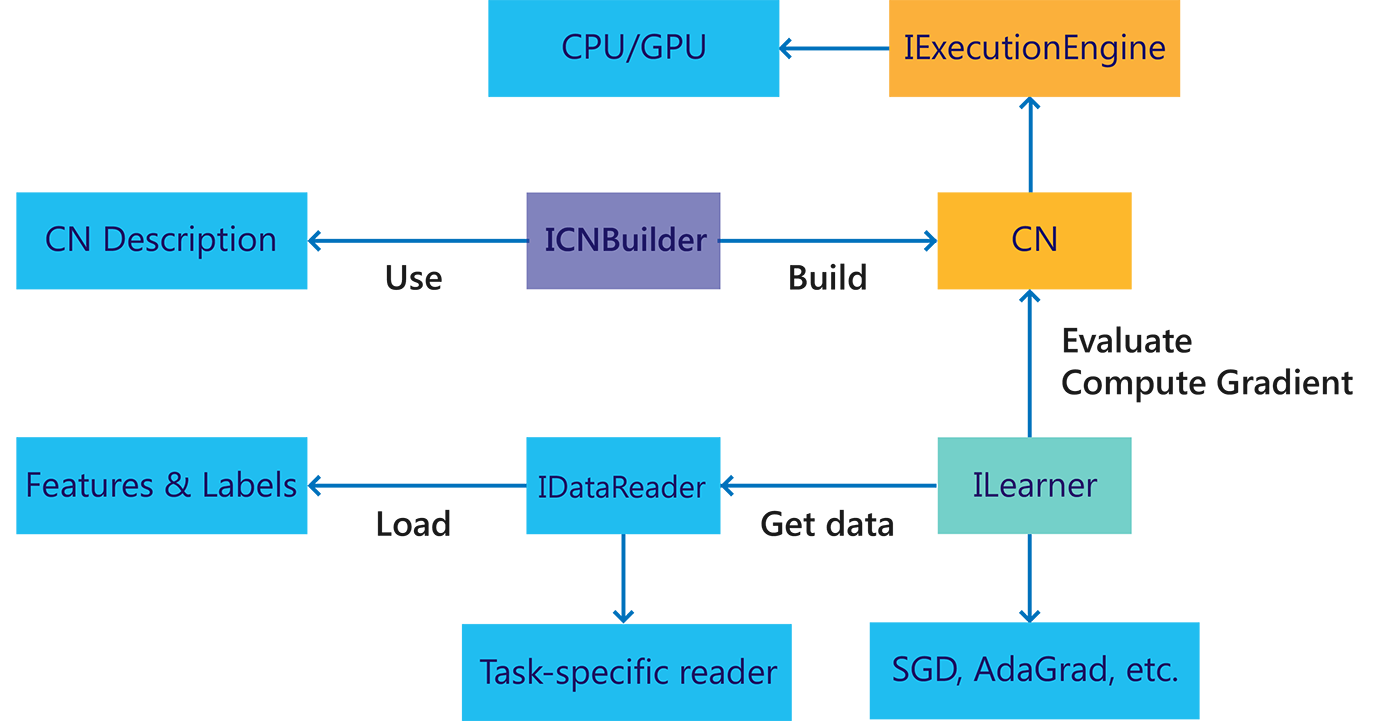
\includegraphics[width=1\textwidth]{pictures/ml_cntk_architecture}
	\caption{\acrshort{cntk} architecture \cite{ml_cntk}}\label{fig:ml_cntk_architecture}
\end{figure}

Thanks to architecture it is very flexible, allows distrubted training and supports main programming languages but lack visualizations.

\section{Apache Spark MLlib}

MLlib\cite{ml_spark} is Apache Spark's scalable machine learning library.

Common\cite{ml_spark_advantages]} problem of prototyping in Python or R is that moving from development to production environments requires extensive re-engineering. 

For this Spark provides data engineers and data scientists with a powerful, unified engine that is both fast (100x faster than Hadoop for large-scale data processing) and easy to use. This allows data practitioners to solve their machine learning problems interactively and at much greater scale.\\

The advantages of MLlib’s design include:

\begin{itemize}[nosep]
\item Simplicity
- Simple APIs familiar to data scientists coming from tools like R and Python. Novices are able to run algorithms out of the box while experts can easily tune the system by adjusting important knobs and parameters.
\item Scalability
- Ability to run the same \acrshort{ml} code on your laptop and on a big cluster seamlessly without breaking down. This lets businesses use the same workflows as their user base and data sets grow.
\item Streamlined end-to-end
- MLlib is on top of Spark and it makes possible to tackle these distinct needs with a single tool instead of many disjointed ones. The advantages are lower learning curves, less complex development and production environments, and ultimately shorter times to deliver high-performing models.
\item Compatibility
- Data scientists often have workflows built up in common data science tools, such as R, Python and so on. MLlib provides tooling that makes it easier to integrate these existing workflows with Spark. 
\end{itemize}


\begin{figure}[h!]\centering
	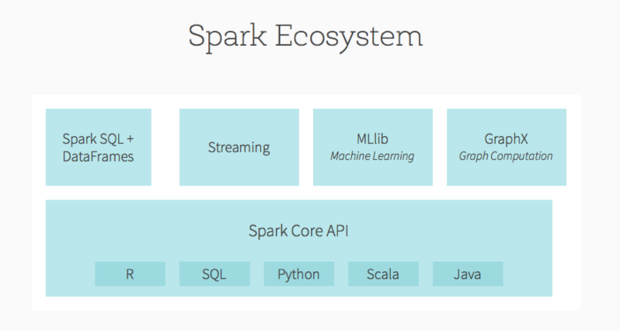
\includegraphics[width=1\textwidth]{pictures/ml_spark_ecosystem}
	\caption{Spark ecosystem \cite{ml_spark_advantages}}\label{fig:ml_spark_ecosystem}
\end{figure}
\pagebreak
\section{MxNet}

Along\cite{ml_mxnet} side previous frameworks Apache's MxNet is a modern open-source deep learning framework used to train, and deploy deep neural networks supporting multiple programming languages.

Supports an efficient deployment of a trained model to low-end devices for inference, such as mobile devices, IoT devices, Serverless or containers which should used the models trained on a higher-level environments because of limited CPU an RAM resources.\\

It has been chosen by \acrshort{aws} be part of their \acrshort{ml} on demand infrastructure.

Now let's switch to some specific algorithm.

\section{Latent Dirichlet allocation}\label{lda_algotithm}

\acrshort{lda}\cite{ml_lda} is a type of topic modeling algorithm. The purpose of \acrshort{lda} is to learn the representation of a fixed number of topics, and given this number of topics learn the topic distribution that each document in a collection of documents has.

In \acrshort{lda}, each document may be viewed as a mixture of various topics. The sparse Dirichlet priors encode the intuition that documents cover only a small set of topics and that topics use only a small set of words frequently. In practice, this results in a better disambiguation of words and a more precise assignment of documents to topics. 

\begin{figure}[h!]\centering
	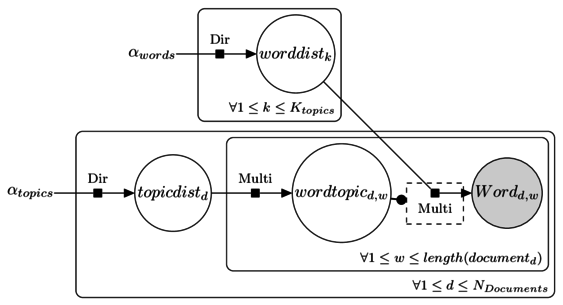
\includegraphics[width=1\textwidth]{pictures/ml_lda_scheme}
	\caption{Plate notation (Bayesian inference) for \acrshort{lda} \cite{ml_lda_exmplanation}}\label{fig:ml_lda_scheme}
\end{figure}

First we need to select number of topics to discover. \acrshort{lda} will go through each of the words in each of the documents, and it will randomly assign the word to one of the K topics. After this step we will have topic representations (how the words are distributed in each topic) and documents represented in terms of topics. This random form is not very optimal or accurate. To better this representation \acrshort{lda} will analyze per document what is the percentage of words within the document that were assigned to a particular topic. And for each word in the document, \acrshort{lda} will analyze over all the documents, what is the percentage of times that particular word has been assigned to a particular topic.

\chapter{Polarion's use cases for ML}

\acrshort{polarion} serves for customers to plan and evaluate their every day work and if something is used frequently and periodically then there should be places for \acrshort{ml} to improve it. Let's find some use cases that can be good candidates for \acrshort{ml}. 

\section{OCR for image attachments}

\acrshort{polarion} allows users to upload files on work items (see the picture below \ref{fig:polarion_attachments}) In current image files are treated without processing their contents and it has impact on functions like search engine that can not use information in files. For this case \acrshort{ocr} should server well.

\begin{figure}[h!]\centering
	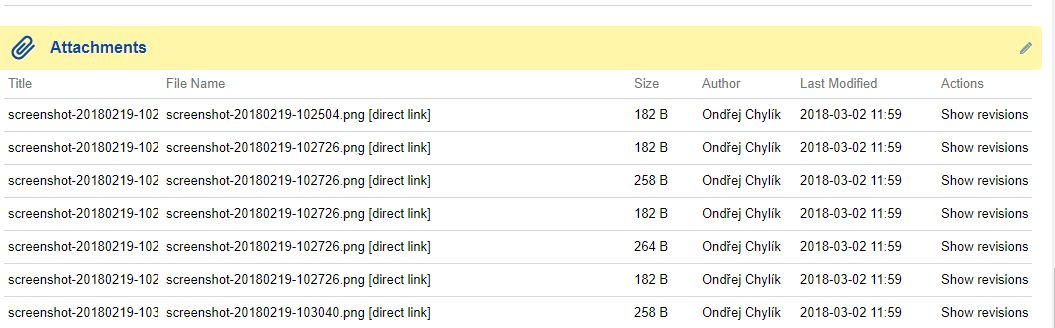
\includegraphics[width=1\textwidth]{pictures/polarion_attachments}
	\caption{Attachments in \acrshort{polarion}}\label{fig:polarion_attachments}
\end{figure}

What is \acrshort{ocr}? \acrshort{ocr} is a technology that enables you to convert different types of documents, such as scanned paper documents, PDF files or images captured by a digital camera into editable and searchable data. \\

Advantages is plenty of free \acrshort{ocr} libraries in variety of programming languages ready to integrate with \acrshort{polarion}. Cost of this implementation should not be high but will lead to an increase in the index size that can rise rapidly as users using attachments a lot.  

\section{Advanced Search in Polarion}

Common problem with large amount of objects is to find that you are searching for. \acrshort{polarion} contains such large amount of objects. For example customers have more than 10 000 different kind of work items and you have to know how to find the specific one. This should be improved no looking just for exactly same expressions but also for similarities and make suggestions based on input data. 

\begin{figure}[h!]\centering
	
\includegraphics[width=1\textwidth]{pictures/polarion_search}
	\caption{Search work item in \acrshort{polarion}}\label{fig:polarion_search}
\end{figure}

Work item's data can contains more specific test like references to another work items, pictures, graphs, stack traces...all these data types should be treated differently. Implementation will be hard as requirements are more unclear but results will lead to improve user experience and less domain experts knowing entire domain and so all work items will be needed.

\section{Suggestion for optimization of Polarion configuration} 

Each customer has a special demands and has a specific environment where \acrshort{polarion} runs on. Optimize these configuration is not easy task as only experts across multiple domains (DevOps, Polarion administrators, Polarion experts, \dots) can see impact and consequences of different settings. \\

This can be changed by us as we know wide range of cases where \acrfull{polarion} or customer was stucked and needed help. This experience contains looking into log for a specific behaviour of user cases, memory/CPU/space/\dots consumption of \acrshort{polarion} or environment itself. Based on this data we should be able to automatically recommend changes to configuration or at least to start resolving problem more proactively before it becomes critical.\\

Example of log information:
\begin{spverbatim}
2018-05-09 15:09:34,595 [main | u:p] INFO  TXLOGGER  - Summary for 'Platform startup': transactions: 0, DB: 20.1 s 
[97% execute (1341x)] (1575x)
2018-05-09 15:09:35,347 [main | u:p] INFO  TXLOGGER  - Summary for 'Context recognition': transactions: 0, svn: 0.436 s [49% getDir2 content (6x), 36% info (8x)] (15x)
2018-05-09 15:09:54,556 [LowLevelDataService-contextInitializer-3 | u:p] INFO  TXLOGGER  - Summary: Total: 19.2 s, CPU [user: 1.25 s, system: 1.06 s], Allocated memory: 440.6 MB, transactions: 0, svn: 10.7 s [92% log2 (25x)] (428x), ObjectMaps: 1.59 s 
[80% setLastProcessedRevision (451x)] (20180x)
2018-05-09 15:09:54,556 [LowLevelDataService-contextInitializer-5 | u:p] INFO  TXLOGGER  - Summary: Total: 19.2 s, CPU [user: 5.61 s, system: 0.859 s], Allocated memory: 3.5 GB, transactions: 0, svn: 8.56 s [61% info (3043x), 28% getFile content (2015x)] (5093x), 
ObjectMaps: 1.78 s [67% saveIfNeeded (24679x), 
11% getPrimaryObjectLocation (6704x), 
11% addLocation (13528x)] (121868x)
2018-05-09 15:09:54,556 [LowLevelDataService-contextInitializer-1 | u:p] INFO  TXLOGGER  - Summary: Total: 19.2 s, CPU [user: 0.891 s, system: 1.25 s], Allocated memory: 461.9 MB, transactions: 0, 
svn: 12 s [94% log2 (45x)] (554x), ObjectMaps: 1.56 s 
[77% setLastProcessedRevision (510x), 15% saveIfNeeded (5391x)] 
(19414x)
2018-05-09 15:09:54,556 [LowLevelDataService-contextInitializer-4 | u:p] INFO  TXLOGGER  - Summary: Total: 19.2 s, CPU [user: 1.11 s, system: 1.5 s], Allocated memory: 596.0 MB, transactions: 0, svn: 13 s [67% log2 (65x), 14% log (1x)] (1445x), ObjectMaps: 1.3 s [72% setLastProcessedRevision (359x), 18% saveIfNeeded (6218x)] (22872x)
2018-05-09 15:09:54,556 [LowLevelDataService-contextInitializer-2 | u:p] INFO  TXLOGGER  - Summary: Total: 19.2 s, CPU [user: 1.55 s, system: 1.8 s], Allocated memory: 705.2 MB, transactions: 0, svn: 13.6 s [88% log2 (56x)] (875x), ObjectMaps: 1.94 s 
[79% setLastProcessedRevision (582x), 11% saveIfNeeded (8406x)] 
(31707x)
2018-05-09 15:09:54,581 [main | u:p] INFO  TXLOGGER  - Summary for 'Context initialization': transactions: 0, svn: 57.9 s 
[74% log2 (216x), 15% info (4897x)] (8395x), ObjectMaps: 8.17 s 
[61% setLastProcessedRevision (1915x), 26% saveIfNeeded (49771x)] (216041x)

\end{spverbatim}
\end{spverbatim}

\section{Suggesting of how to split a document Space} \label{sec:lda_case}

\acrshort{polarion} is about working with documents. It is expected that customers have a hundreds of documents separated into document spaces. Document spaces are used as folders and make hierarchy. But in some cases customers create too many document under one document space and orientation within this space becomes unclear. Idea is to split documents under one document space into groups based on their topic. This is a job for \acrshort{lda}.

\begin{figure}[h!]\centering
	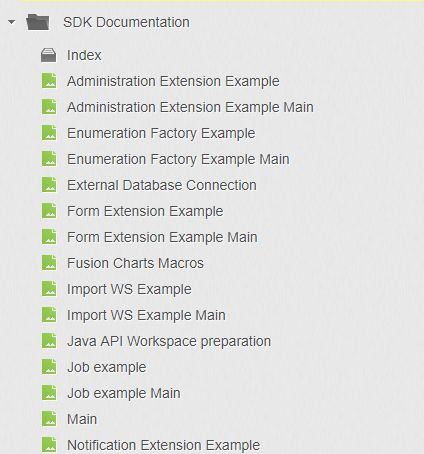
\includegraphics[width=1\textwidth]{pictures/polarion_document_space}
	\caption{Document space in \acrshort{polarion}}\label{fig:polarion_document_space}
\end{figure}

As was said before \acrshort{polarion} document contains beside plain text also its work items that contain its own text including title, description, comments, selected properties... All these information should be taken into account for topic creation. Work item can have a reference to another work item and so on that is question how many work items in such chain use. 

Welcome topics into \acrshort{polarion} improves user experience on every day basis. If we talk about splitting documents in one document space topics can be also created for all documents and users will be able to find similar document across entire \acrshort{polarion} which is normally really hard task to do.

\acrshort{lda} is downloadable library and can be easily integrated into existing code base. Changes on the side of \acrshort{polarion} will be much harder but business value of this feature is good enough to balance it.

\section{Translating documents}

Normally customers have all their documents in one language. But there are cases when a document is created in one language and from the document is branched to another one which is translated to different language needed for example for external communication.\\

Important note is that a source document and a branched document are connected together and so changes to one can be propagated to another. Direction of propagation should be only from source to branched document because it is expected that branched document will contain more information than its source. First translation when branched document is created has no problems but complications come when the source is changed and changes should be propagated to its branched documents. These documents can already have overwriting or context changing changes and the question is how to solve a collision issue. \\

Anyway problem lies also in translation itself though translation services are widely accessible we can not sent customer's data outside their environment and local translation server must be used.

\section{Estimations and expectations}

Agile planning is built around task estimation, fulfilling expectations and constant improving by learning from estimations. The more experienced developer is, the better estimates has. Average time for a programmer job is in order of years and time to take familiar with \acrshort{polarion} is more than year. That is why estimates from inexperienced programmer are more tips then relevant data. On the other hand \acrshort{polarion} has previous data from all project done before which may give hints with the estimation of a task.\\ 

Firstly we need to find similar tasks. We can look for work items with same parameter like category, story type and so on and combine it with similarity of description. Process all estimations from these found work items and show to user advice what estimate should be used.

\begin{figure}[h!]\centering
	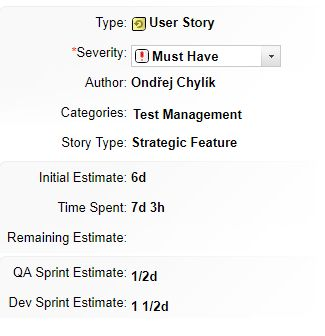
\includegraphics[width=1\textwidth]{pictures/polarion_estimation}
	\caption{Estimations in \acrshort{polarion}}\label{fig:polarion_estimation}
\end{figure}

\section{Defect recommendations} \label{sec:defect_recommendations}

Defect is a special type of work item in \acrshort{polarion} using to track errors and misbehaviours of the system. Creating of this type is done by whoever found the defect and so the author need to have knowledge about already created defects and how to correctly set all parameters for that type of defect. \acrshort{polarion} can try to find similar defects and help the user to better set properties up.\\

\begin{figure}[h!]\centering
	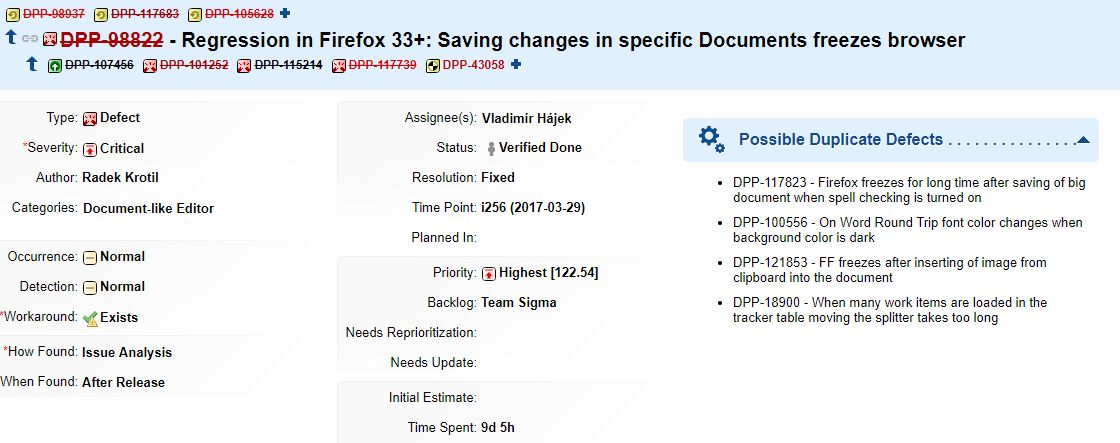
\includegraphics[width=1\textwidth]{pictures/defect_menu}
	\caption{Properties of defect work item  in \acrshort{polarion}}\label{fig:defect_menu}
\end{figure}

Similar defects will be searched based on title of the defect that is written by a author and must be so accurate information as possible to ensure better results. \\

\pagebreak

Properties for recommendations:
\begin{itemize}[nosep]
\item severity
\item priority
\item assignee
\item package
\item category\\
\end{itemize}

Thanks to this defects will get faster to the responsible person and the time from finding to the first reaction or even fix will be significantly shorter. It has clear business values helps entire company to react faster and with less people to be involved.

\section{Chat bot}

For such a huge product as \acrshort{polarion} is it is natural that users are sometimes lost. Whether it's forgotten of old stuff or looking for new functions or processes. In both cases they have two options. The first is to try search on \acrshort{polarion} help page\ref{polarion_help} and the second is to bother a colleague. It is true that the better they know the question they get the answer faster and here can help chat bot.\\

\begin{figure}[p!]\centering
	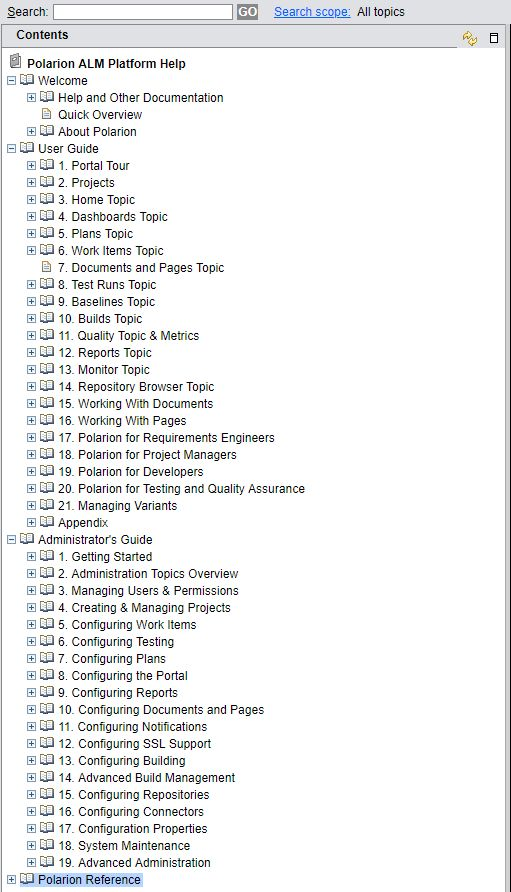
\includegraphics[width=1\textwidth]{pictures/polarion_help}
	\caption{Help page in \acrshort{polarion}}\label{fig:polarion_help}
\end{figure}

Idea is to take existing help page and index it in a usable format for some of the open-source chat bots. This first line of communication will help users to solve their problems separately and questions to colleagues or even Polarion experts will be reduced leading to more productivity environment.  

\section{The most complained parts of Polarion}

\acrshort{polarion} accepts complaints and suggestions every day from wide range of customers. As a results new projects are emerging to add new functionality or to fix the old ones to better satisfy customer's demands poorly analyzed during the first implementation. Creating of new project is done by a management who would like to welcome a tool to track specific parts of \acrshort{polarion} mostly targeted by customer's demands.\\

We need to take into account not only information but also its sentiment how much is a customer concerned with this problem. 	

\section{Detection of duplicated defects}

Many new defects are created every day. The standard process describes that before the creation, the user should verify that the same defect does not exists. This is done by searching \acrshort{polarion} and as was said previously it is not as good as should be also because there is no specific specification as to what the new defect should look like and how it should contain information.\\

\acrshort{polarion} already contains basic duplicate analysis show on \ref{fig:polarion_defect_similar}.

\begin{figure}[h!]\centering
	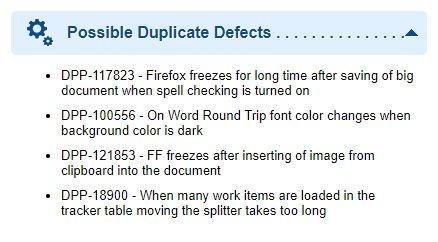
\includegraphics[width=1\textwidth]{pictures/polarion_defect_similar}
	\caption{Similar defect suggestion in \acrshort{polarion}}\label{fig:polarion_defect_similar}
\end{figure}

Analysis of duplicates should be extend to more complex form taking in account also reference work items, similar but not the same text, attachments and so on.

\chapter{Proof of concept prototypes}

We go through \acrshort{ml} frameworks and algorithms and useful \acrshort{polarion} user cases expandable with \acrshort{ml}. Now it is time to come with \acrshort{pof} prototypes for some of the previous user cases.\\

From internal discussion came up these two user cases:
\begin{itemize}[nosep]
\item Suggesting of how to split a document Space\ref{sec:lda_case}
\item Defect recommendations\ref{sec:defect_recommendations}
\end{itemize}

Let's move on to their implementation done in a team.

\section{Prototype - suggesting of how to split a document Space}

Task to split documents is a task to find their topics a group them with them. Finding topics is a perfect task for the previously mentioned \acrshort{lda}\cite{lda_algotithm} algorithm. 

Technologies used:
\begin{itemize}[nosep]
	\item PostgreSQL
	\item Java
	\begin{itemize}[nosep]
		\item Spring
		\item LDA from \url{https://github.com/chen0040/java-lda}
	\end{itemize}[nosep]
	\item D3 Data Driven documents\cite{d3}
\end{itemize}[nosep]

The procedure is as follows:
\begin{enumerate}[nosep]
\item data acquisition and clearing
\item creating topics
\item visualisation\\
\end{enumerate}

For \acrshort{pof} purposes no integration with \acrshort{polarion} code base will be done. 

\subsection{data acquisition}

It is possible to get data form \acrshort{polarion} through its API. But our case required to download data directly from database when data are stored to own database used just for the prototype. For this purpose the production database were cloned and used.\\

First step is to download all documents data. Then process each document's description and get list of work items contained in the document and download them. After it go through newly downloaded work items and look into their description for a references work items. If there is a referenced work items and download them if the work item was not downloaded previously.\\ 

Some problems were encountered:
\begin{enumerate}[nosep]
	\item Document has invalid data
	- reason for this are mainly historical data and these documents were skipped.
	\item Incorrect referenced URL
	- link to referenced work item is in invalid format. Again reason for this is a historical form of link and these links were skipped. 
	\item Non existing work items
	- can happen and links were skipped
\end{enumerate} 

After application of these restriction we have thousands of documents with tens of thousands work items ready to next stage.

\subsection{creating topics}  

This is where \acrshort{lda} library is coming to the scene.

Firstly we need to convert document data to just a plain text suitable for \acrshort{lda}. This processing takes text from document including its title and connects it with text from all his work items. Text from work items again means title plus description and if there is a referenced work item also text from it.\\

Processing is done in 4 levels when for the first level all documents are taken, topics generated. 5 most common topics are taken a documents suitable for them are put under them. Next level takes just a document under one topic a do the same thing as in previous step and so on for the next levels. Results is a three chart structure of all documents in \acrshort{polarion}\ref{lda_tree_chart}.\\

First runs revealed problem with interpretation of words so these sets were defined: 
\begin{itemize}[nosep]
 \item stop words - common words used in language without specific meaning - ignored
 \item html - html tag commonly used in work item's description but inappropriate for topics modeling - ignored
 \item Polarion keywords - keywords from Polarion domain like \textit{workitems},\textit{dpp}, \textit{wiki} and so on - ignored
 \item special - command words like \textit{while} or \textit{for} - ignored\\
\end{itemize}

\begin{figure}[h!]\centering
	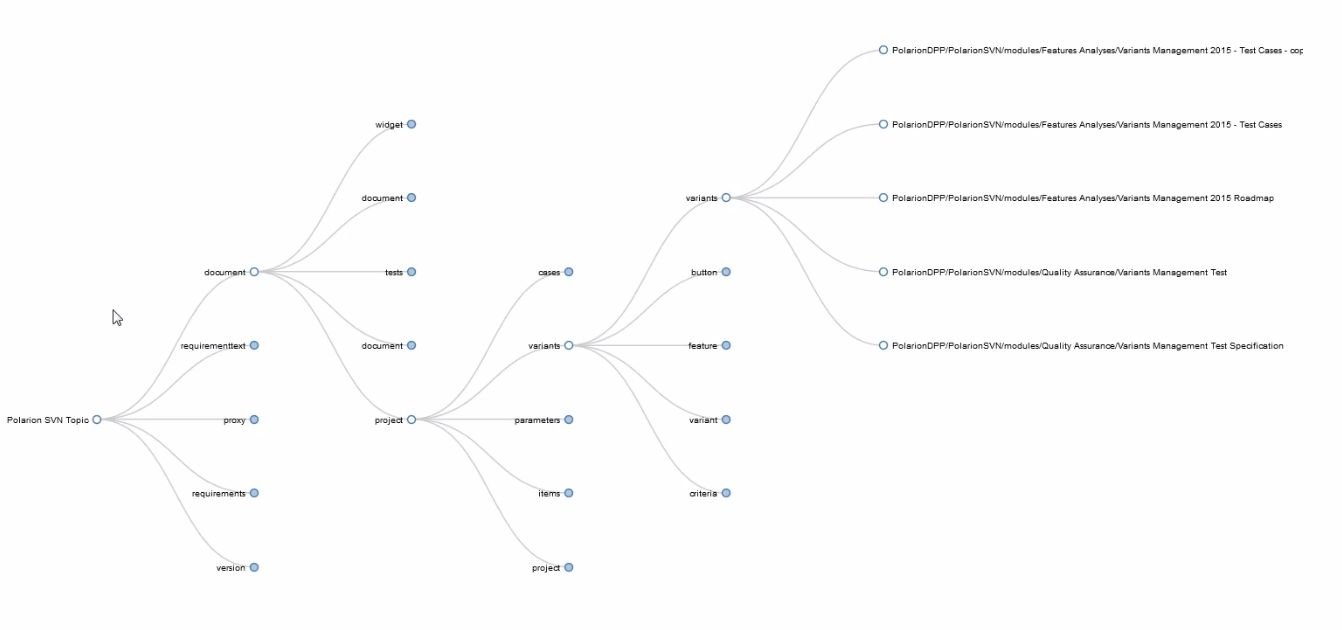
\includegraphics[width=1\textwidth]{pictures/lda_tree_chart}
	\caption{Tree chart of documents}\label{fig:lda_tree_chart}
\end{figure}

Using \acrshort{lda} library works flawlessly without any stuck or unexpected behaviour.   

\subsection{Visualisation} 

Using \acrshort{d3} library provides nice and easy to use visualizations. 

Showing the most common topics for documents. More bigger the topic name is, the more topic is common in the documents. You can recognize that some names are redundant it is because topics were named after their most common word. See pictures below \textit{Topics distribution in external database documents}\ref{fig:lda_topics_external_database} and \textit{Topics distribution in variant management documents}\ref{fig:lda_topics_vm}.\\
	   
\begin{figure}[p!]\centering
	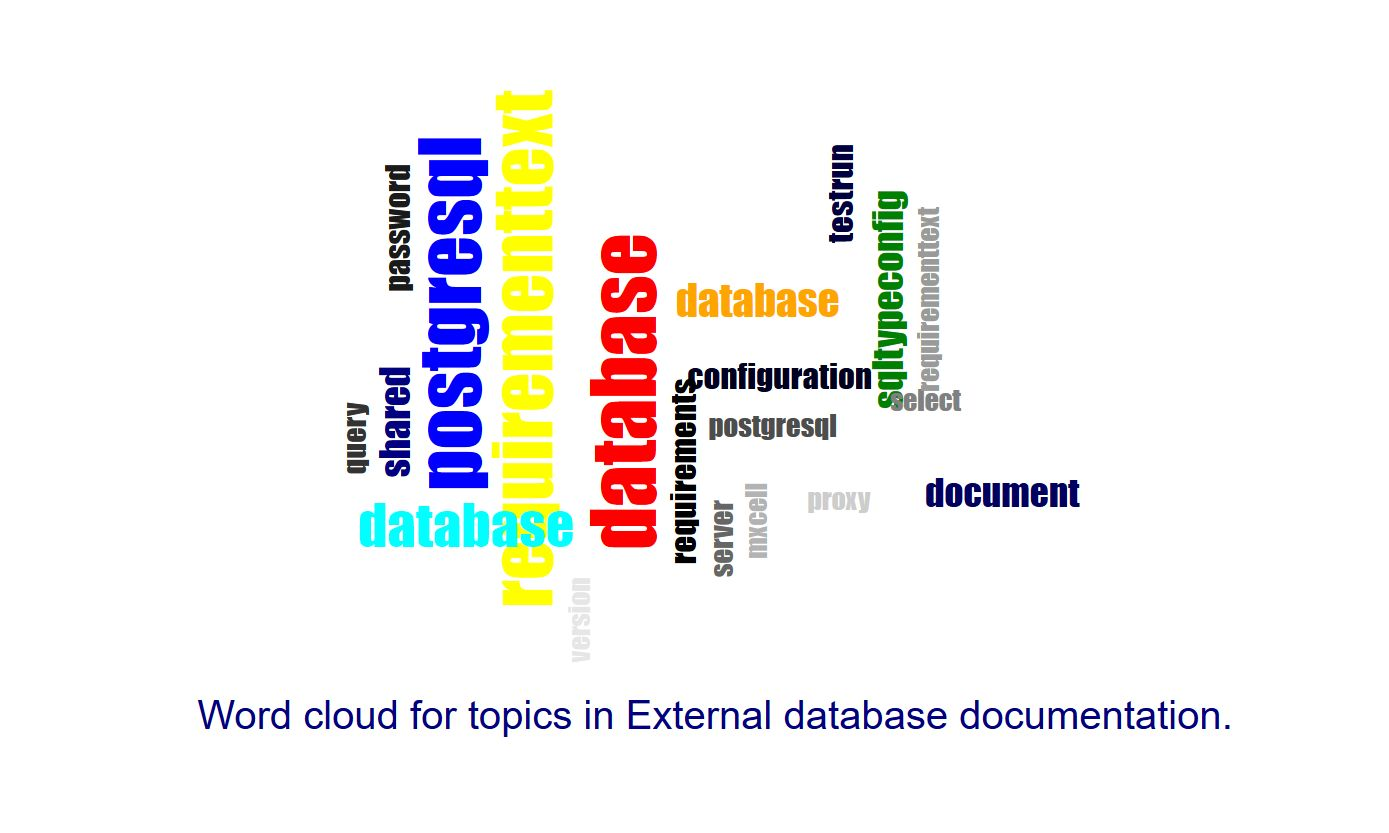
\includegraphics[width=1\textwidth]{pictures/lda_topics_external_database}
	\caption{Topics distribution in external database documents}\label{fig:lda_topics_external_database}
\end{figure}

\begin{figure}[p!]\centering
	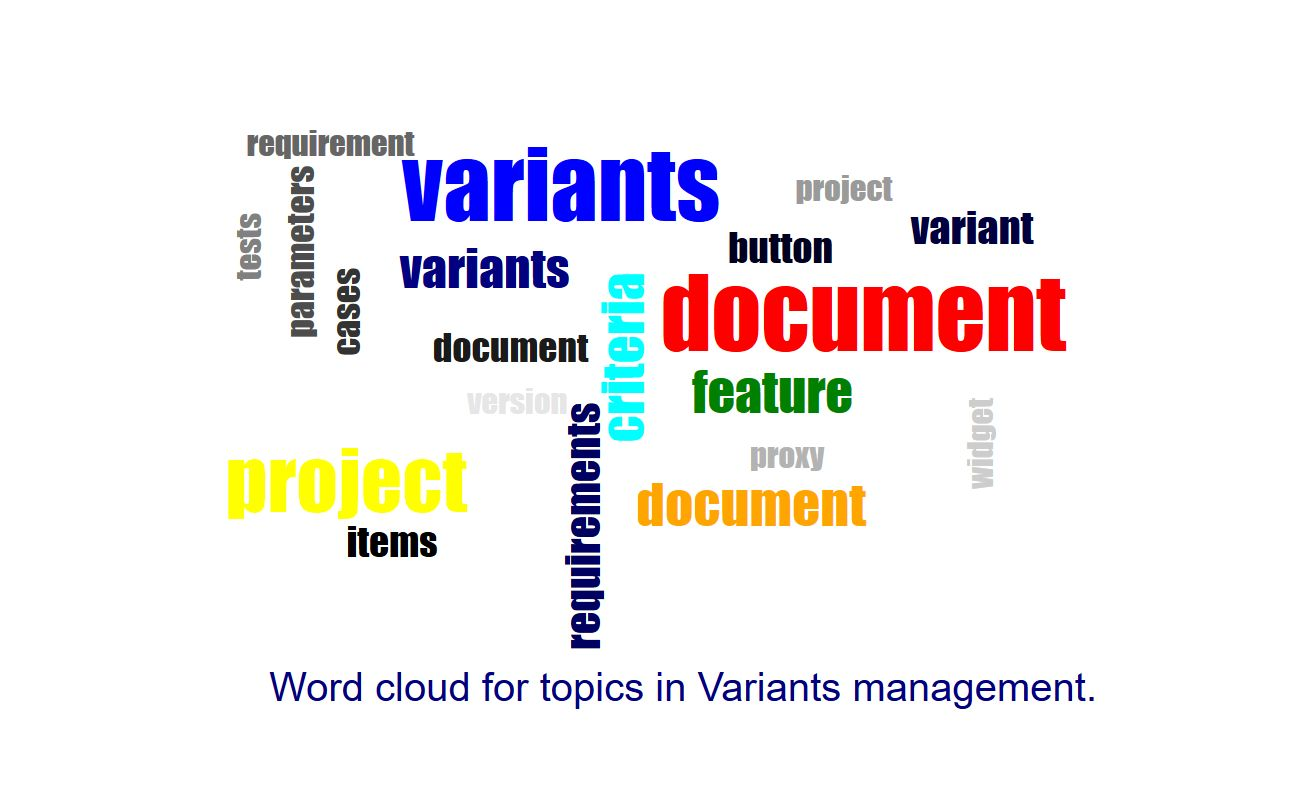
\includegraphics[width=1\textwidth]{pictures/lda_topics_vm}
	\caption{Topics distribution in variant management documents}\label{fig:lda_topics_vm}
\end{figure}

Impressive visualization is a circle graph of all topics. It is circle view of previous tree chart where white circles are documents and depending on how big the white circle is, as a matter of fact, belongs to the topic. See \textit{Circle representation of all topic}\ref{fig:lda_documents_cloud} and \textit{Detail of topics in circle representation}\ref{fig:lda_circle_detail}.

\begin{figure}[h!]\centering
	
\includegraphics[width=1\textwidth]{pictures/lda_documents_cloud}
	\caption{Circle representation of all topics}\label{fig:lda_documents_cloud}
\end{figure}

\begin{figure}[p!]\centering
	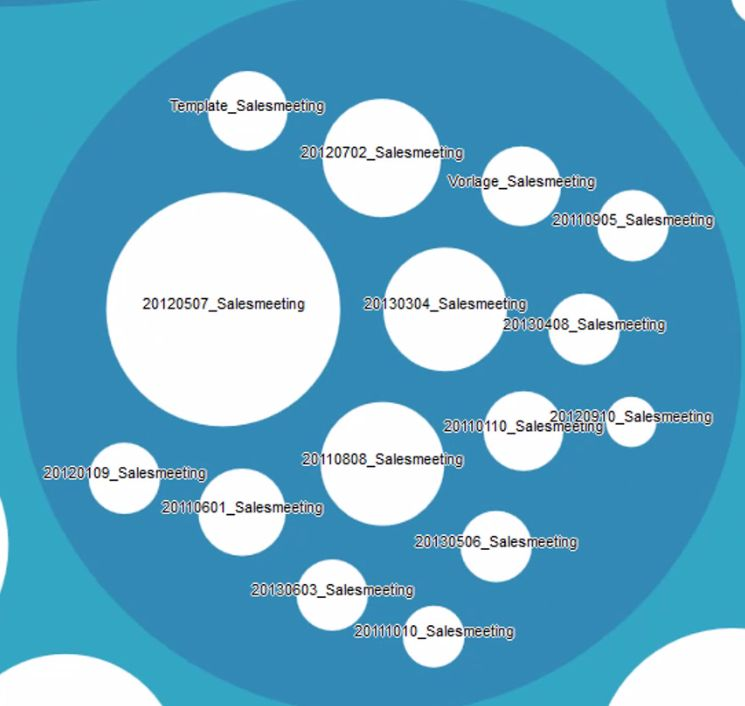
\includegraphics[width=1\textwidth]{pictures/lda_circle_detail}
	\caption{Detail of topics in circle representation}\label{fig:lda_circle_detail}
\end{figure}

\pagebreak
\clearpage
\section{Prototype - defect recommendations}\label{prototype_defect_rec}

\acrshort{aws} was used for \acrfull{ml} implementation providing interface for data modeling in a form what is needed. Author also had a previous experiences and participate in the training around \acrfull{aws} helping him to realize this prototype faster. \\

What was used:
\begin{itemize}[nosep]
\item \acrshort{aws} cloud service and its own ML/AI engine.
\item \acrshort{aws} provides a service to import data, store, train ML engine, and setup learning and ML service to cater to specific data sets. 
\item SCALA was used for a back-end and for extracting and pushing data from \acrshort{polarion} to \acrshort{aws}.
\item JavaScript injection via Chrome extension was used to inject JS/HTML into a \acrshort{polarion} UI so you can see the results.
\item Asynchronous real-time connection between \acrshort{polarion} UI, SCALA back-end and \acrshort{aws} was used as a connection.\\
\end{itemize}

5 categories were selected to recommendation:
\begin{itemize}[nosep]
	\item Assignee
	\item Priority
	\item Severity
	\item Category
	\item Package\\
\end{itemize}

Two separated parts were implemented:
\begin{itemize}[nosep]
	\item Loading Polarion defect data
	\item Real-time pull of results based on Polarion input\\
\end{itemize}

\subsection{Loading Polarion defect data}

Data was downloaded from \acrshort{polarion} services and processed to \acrshort{aws} cvs input format. Example of such a data file is below. In reality file has thousands and thousands of lines.

\begin{spverbatim}
id,title,assignee,priority,severity,linkedRevisions
DPP-10188, linking a particular historical revision of a wiki 
page does not work,Pavel Borovik,105.35,blocker,186728
DPP-10188, linking a particular historical revision of a wiki 
page does not work,Pavel Borovik,105.35,blocker,191862
DPP-10110,Polarion program shortcuts do not works since Polarion 
3.3 when updated from previous version,Jiri Banszel,60.35,major,
188587
DPP-10212,Export of formatted multi-lined text to Excel table 
fails with ClassCastException,Jiri Banszel,82.35,critical,186439
\end{spverbatim}
\end{spverbatim}
\bigskip
Then data file where pushed as a \textit{AWS ML data set} into a \acrshort{aws} cloud for \acrshort{ml}. ML uses 70 \% of data to learn and then it test itself by using the rest (30 \%) and provides a probability of its guesses by express it in \%.\\

For each category was created one file and from this file one endpoint as so for each category estimation implementation consumes different endpoint.

\subsection{Real-time pull of results based on Polarion input}

Basic description is that user enters title of work item and click on \acrshort{ml} bar to show recommendations. Communication scheme is shown in the picture \textit{Communication scheme}\ref{fig:defect_bot_scheme}.\\

\begin{figure}[h!]\centering
	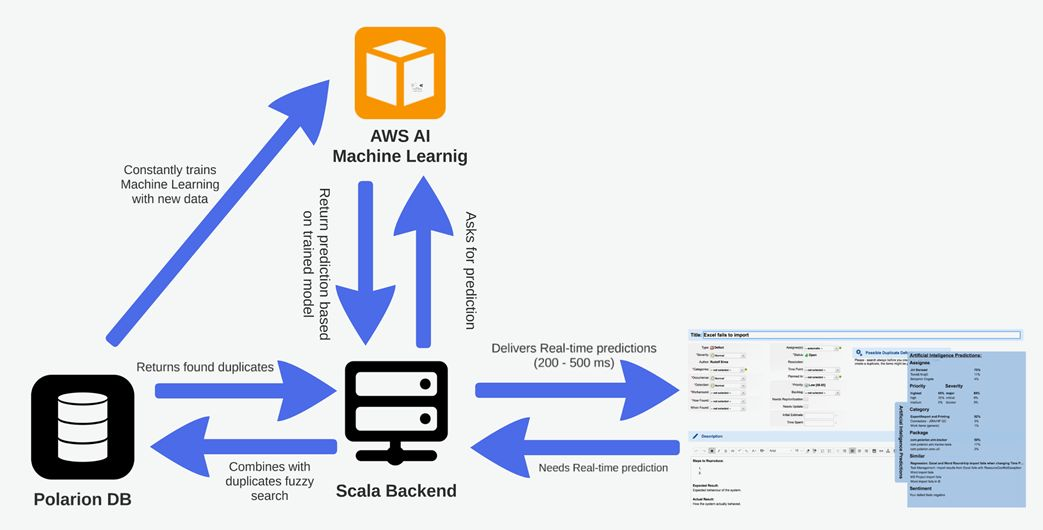
\includegraphics[width=1\textwidth]{pictures/defect_bot_scheme}
	\caption{Communication scheme}\label{fig:defect_bot_scheme}
\end{figure}

\begin{enumerate}[nosep]
	\item User enters a title and request recommendations
	\item Chrome extension grab title and send it to scala backend
	\item Scala backend asks \acrshort{aws} for recommendations and returns it to chrome extension
	\item Chrome extension shows recommendations to user as shown in the picture below \ref{fig:defect_bot_workitem}\\
\end{enumerate}

\begin{figure}[h!]\centering
	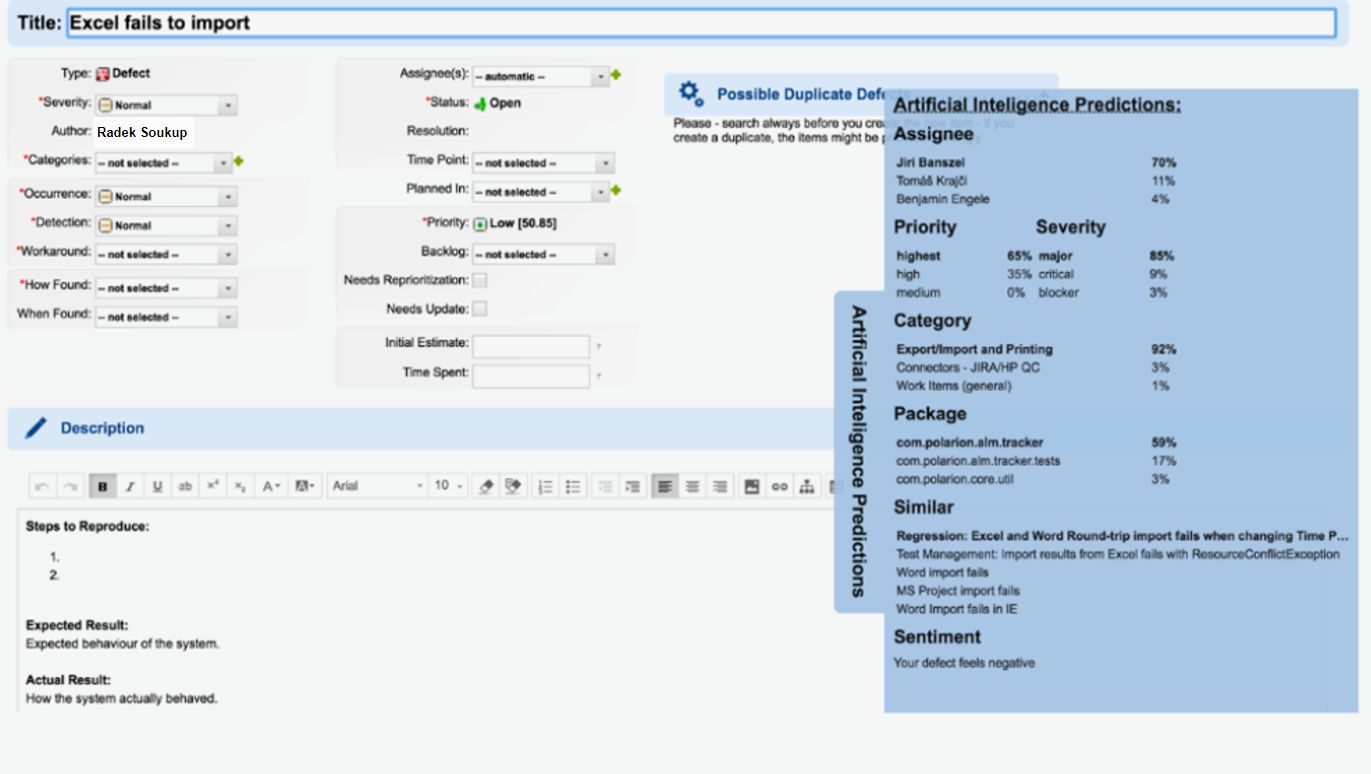
\includegraphics[width=1\textwidth]{pictures/defect_bot_workitem}
	\caption{Practical use}\label{fig:defect_bot_workitem}
\end{figure}

Quality of the results is surprisingly good and shows great potential for future production implementation. System is currently deployed on testing environment ready to be extended.

\chapter{ML in Polarion production}

Both implemented prototypes are in test environment ready for further development together with not implemented ideas that are still on table. Decision to go to production is not so simple as can look like because if your product operate in a regulated environment any violation against these regulation may have fatal impact on \acrshort{polarion} trade mark. The main problem are data and customers must be sure that with data being handled correctly all the time. \\ 

Let's look at \acrshort{gdpr} regulation coming into force just these days when this thesis is published.

\subsection{General Data Protection Regulation}

Data are fuel for \acrshort{ml} but their use can be limited especially if we talk about customer's data with sensitive information. Now we face new regulation in form of \acrshort{gdpr} that will change rules how to threat and store data. What \acrshort{gdpr} is?\\

\acrshort{gdpr}\cite{gdpr_info} is a legal framework that sets guidelines for the collection and processing of personal information of individuals within the European Union (EU). Thse \acrshort{gdpr} sets out the principles for data management and the rights of the individual, while also imposing fines that can be revenue-based. The General Data Protection Regulation covers all companies that deal with data of EU citizens, so it is a critical regulation for corporate compliance officers at banks, insurers, and other financial companies. \acrshort{gdpr} will come into effect across the EU on May 25, 2018.\\

Data types affected by \acrshort{gdpr} are:
\begin{itemize}[nosep]
\item Basic identity information such as name, address and ID numbers
\item Web data (location, IP address, cookie data, \dots)
\item Health and genetic data
\item Biometric data
\item Racial or ethnic data
\item Political opinions
\item Sexual orientation\\
\end{itemize}

What companies will be affected by:
\begin{itemize}[nosep]
	\item A presence in an EU country.
	\item No presence in the EU, but it processes personal data of European residents.
	\item More than 250 employees.
	\item Fewer than 250 employees but its data-processing impacts the rights and freedoms of data subjects, is not occasional, or includes certain types of sensitive personal data. That effectively means almost all companies.\\
\end{itemize}

\acrshort{gdpr} extends rights of data subjects that can be summarized like:
\begin{itemize}[nosep]
\item the right to access
\item the right to be forgotten, a.k.a. right to erasure
\item the right to data portability\\
\end{itemize}

In more detail look at the picture below \ref{fig:gdpr_subject_rights}.
\begin{figure}[h!]\centering
	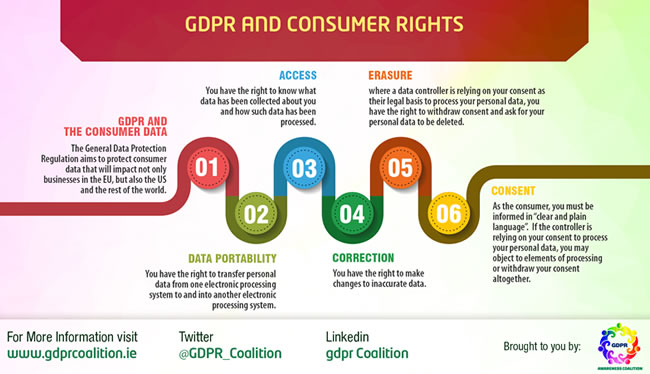
\includegraphics[width=1\textwidth]{pictures/gdpr_subject_rights}
	\caption{\acrshort{gdpr} consumer rights \cite{gdpr_subject_rights}}\label{fig:gdpr_subject_rights}
\end{figure}

\begin{itemize}[nosep]
\item  The data subject’s right of access which means 
	\begin{itemize}[nosep]
	\item  the right to know whether data concerning him or her are being processed and 
	\item  if so, access it with loads of additional stipulations.
	\end{itemize}
\item  The data subject’s right to rectification. When personal data are inaccurate, then controllers need to correct them indeed.
The previously mentioned right to erasure or right to be forgotten with additional stipulations, among others if personal data has been made public.
\item The data subject right to restriction of processing. Simply said, the right of the consumer or whatever you call the natural person under the scope of the \acrshort{gdpr}, to limit the processing of his/her personal data with, once more, several rules and exceptions of course.
\item  The right to be informed. In general, the \acrshort{gdpr} asks controllers and so on to inform data subjects on several matters. Providing clear and correct information is a key duty in many regards. Simply said, the \acrshort{gdpr} wants consumers to know because if you don’t know you can’t decide. The controller must inform recipients who got these data, where feasible. And then the data subject also has a right, even if not strictly called a right, to ask \textit{who are all these recipients who got to see my data}. 
\item  The right to data portability. This is again one of those data subject rights that are in the infographic and which we covered more in depth previously.
\item  The data subject’s right to object. That does indeed mean what it says: data subjects can say they don’t want the personal data processing to be done or going on. Direct marketers and people who do profiling should pay a lot of attention to the right to object as it’s a lot about them and certainly profiling with automated means.
\item  The data subject right not to be subject to a decision based solely on automated processing, including profiling, which produces legal effects concerning him or her or similarly significantly affects him or her.\\
\end{itemize}

\begin{figure}[p!]\centering
	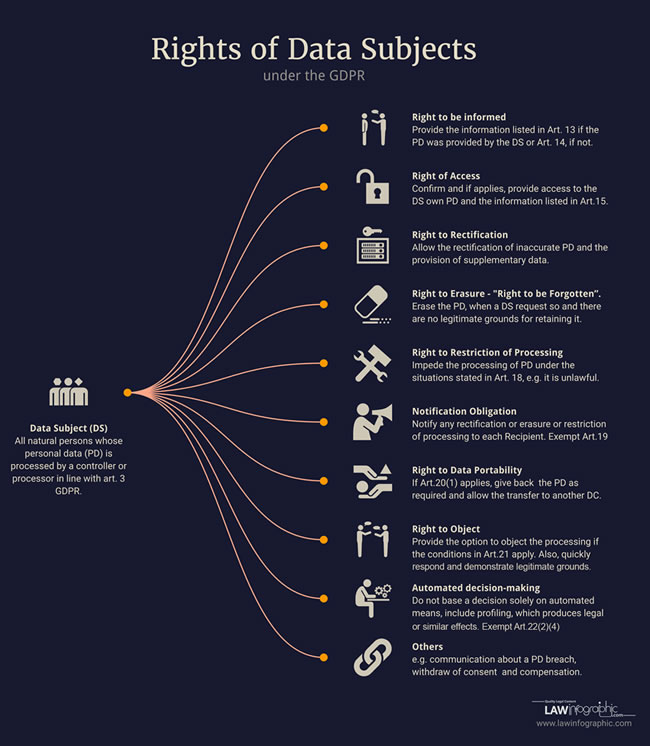
\includegraphics[width=1\textwidth]{pictures/gdpr_subject_rights_detail}
	\caption{\acrshort{gdpr} consumer rights in detail \cite{gdpr_subject_rights}}\label{fig:gdpr_subject_rights_detail}
\end{figure}

What we need to be careful about and is not part of current Data Protection Directive?

\begin{itemize}[nosep]
\item Data breach notification: Controllers and processors are now required to notify supervisory authorities within 72 hours of learning of a breach and to notify the people to whom the data applies \textit{without undue delay}. 
\item Explicit consent: \acrshort{gdpr} requires that at the time you collect personal data, explicit consent must be given by the data subject. This means organisations can no longer bury generic consent in a long form full of legalese. Instead, organisations must offer specific information on what data is collected, how the data will be stored and processed, and must use clear and plain language. Nothing short of opt-in will do, and it must be as easy to withdraw consent as to give it. 
\item Data transfer out of the EU: Personal data must not leave the EU unless you have approval from the supervisory authority, or where the data subject is informed of the data transfer and associated risks and authorises the transfer. 
\item Data protection officer (DPO) appointment: If you process data on a large scale then you must appoint, hire, assign or contract with a DPO, who is your representative to the supervisory authorities that monitor and ensure compliance with the regulation.\\
\end{itemize}

IT with \acrshort{ml} is very competitive environment where companies around the world fight for primacy in research and business use. And as \acrshort{gdpr} affects only EU this can disadvantage EU companies with their world competitors and their moving our of EU borders. Still true impact of \acrshort{gdpr} is unclear and only future shows.\\

For \acrfull{polarion} \acrshort{gdpr} leads to more strictly regulation already so strict environment. Transfer data to external services seems to be quite hard and for this \acrshort{polarion} should implement its own \acrshort{ml} solution that customers can install in their own secured environment and work with it without sending data to external repositories.

\section{ML future}
\acrshort{ml} is no longer in category should have but it quickly move to technology that all system must have in some way and it does not matter if it will voice recognition, chat bot or some sort of data analysis. As you can see in the picture \textit{Expected IT budget for ML}\ref{fig:ml_budget} almost all companies invest in \acrshort{ml} technologies with vision of improving their profit greatly.\\

\begin{figure}[h!]\centering
	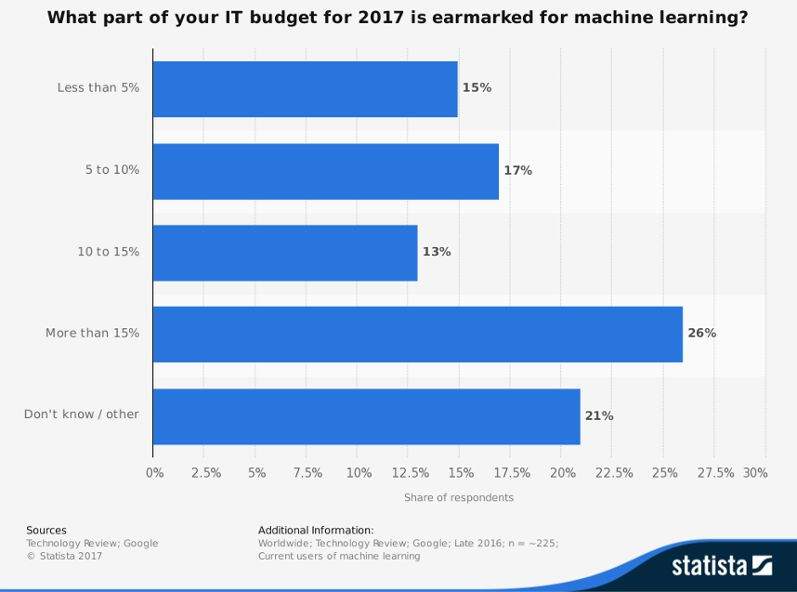
\includegraphics[width=1\textwidth]{pictures/ml_budget}
	\caption{Expected IT budget for ML\cite{ml_realword}}\label{fig:ml_budget}
\end{figure}

Of course \acrshort{ml} is not the only technology changing market and market expectation are seen in the picture \textit{Technologies trends over next 3 years}\ref{fig:ml_changing_market} and \acrshort{ml} experts paid in gold.

\begin{figure}[h!]\centering
	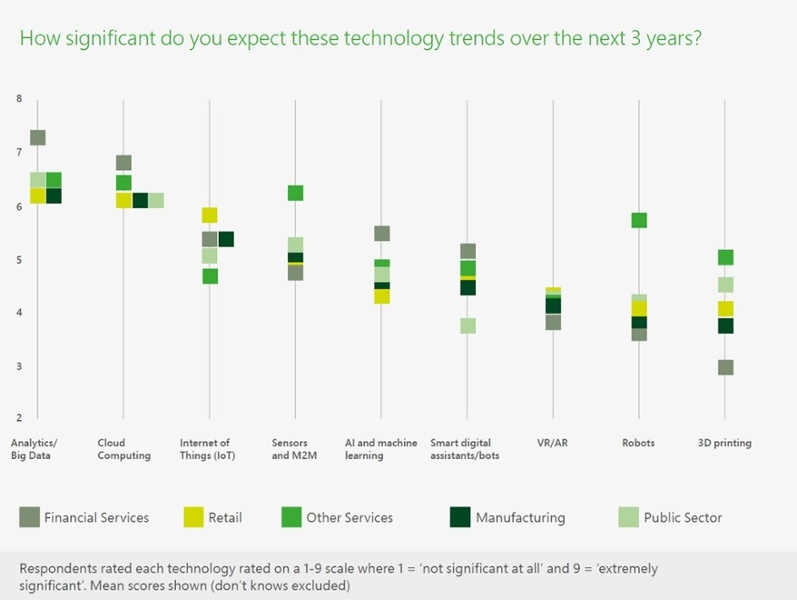
\includegraphics[width=1\textwidth]{pictures/ml_changing_market}
	\caption{Technologies trends over next 3 years\cite{ml_realword}}\label{fig:ml_changing_market}
\end{figure}

Important change is the time from idea to \acrshort{pof} implementation. We are no longer talking about years but more likely months and even weeks or days. And \acrshort{ml} was about pure mathematical algorithms and equals no it is more about integrations of existing \acrshort{ml} solutions and massage it with own data. It helps management to see and recognize benefits \acrshort{ml} projects in their product in a shorter time and with a lower cost and make a decision to start with production implementation.

\section{Changes to environment}

The practical impact of \acrshort{gdpr} on data manipulation is something what will revealed and in current state it is better to wait and see what happens. 

But for sure what we used for Defect recommendation\ref{prototype_defect_rec} can not be used in production environment. We need to move \acrshort{ml} server to \acrshort{polarion} environment by using existing server's implementations or create our own server. \acrshort{ml} community provides libraries and guides helping with creating own server what is our next target.

\begin{conclusion}
	
We have analyzed and described \acrshort{polarion} main parts and benefits what makes \acrshort{polarion} one of the best \acrshort{alm} solution on the market of large enterprise solutions with strong regulations that are reason why user experience is worse in compare with others lightweight solutions. 

Review of \acrshort{ml} existing solutions and algorithms revealed readiness of \acrshort{ml} for a fast prototyping and production deployment. Big companies like Facebook, Google or Microsoft continue with developing their own \acrshort{ml} frameworks with growing community support and production implementations.

We dig deep into \acrshort{polarion} using and found several promising user case candidates for \acrshort{ml} prototyping. Each of these user cases has a valuable business potential move \acrshort{polarion} one step above the competitors without the need for drastic changes to the current implementation.

We have chosen two user cases and successfully implement prototype for each of them. Implementation confirm that prototyping is no longer task for years but rather months or even weeks with \acrshort{ml} services as \acrshort{saas}. both prototypes are now in test environment and ready to next development.  

Despite the fact that prototyping is easier than ever before, move to production remains complicated not only from the point of view technologies, but rather regulation and new \acrshort{gdpr} guideline slow down or even make it impossible.

Nevertheless \acrshort{ml} will be more and more common part of any application and companies have to catch up with this trend to survive. \acrshort{polarion} works on it.   


\end{conclusion}

\bibliographystyle{csn690}
\bibliography{mybibliographyfile}

\appendix

\chapter{List of abbreviations used}

\printglossaries

\begin{description}
	\item[ALM] Application lifecycle management
	\item[Polarion] Polarion ALM
	\item[ML] Machine learning 
	\item[pof] Proof of Concept
	\item[RNN] Recurrent neural network
	\item[AWS] Amazon web services
	\item[GUI] Graphic user interface
	\item[CNTK] Microsoft Cognitive Toolkit
	\item[LDA] Latent Dirichlet allocation
	\item[GDPR] General data protection regulation
	\item[OCR] Optical character recognition
	\item[D3] D3 Data-driven documents
	\item[SaaS] Software as a service
\end{description}

\chapter{CD contains}

\begin{figure}
	\dirtree{%
		.1 readme.txt\DTcomment{stručný popis obsahu CD}.
		.2 thesis\DTcomment{zdrojová forma práce ve formátu \LaTeX{}}.
		.1 text\DTcomment{text práce}.
		.2 thesis.pdf\DTcomment{text práce ve formátu PDF}.
		.2 thesis.ps\DTcomment{text práce ve formátu PS}.
	}
\end{figure}

\end{document}
